\section{Results and Discussion}\label{sec:results}
The following results use the corrected common evaluator and equal-evaluation protocol. The primary weight is $\rho=1$; Section~\ref{sec:rho} reports the Karatsuba-weighted scenario. All values come from the new caches, not the historical experiment.
\begin{table*}[!htbp]
\centering
\caption{Results over 30 independent runs with $\rho=1$: median [interquartile range]. HV: hypervolume of the delivered set (identification or free-run validation error); $C_\tau$, NRMSE$_\tau$: cost and free-run validation NRMSE of the model selected by the $\tau$-rule; Rec.$_\tau$, Rec.$_\mathcal{P}$: fraction of runs in which the selected model, or at least one model of the returned set, contains the three true regressors of \eqref{eq:tutorial}. $^{\ast}$/$^{\dagger}$: Green differs from SO/MO-lex (Mann--Whitney, Holm-adjusted $p<0.05$).}
\label{tab:results}
\footnotesize
\setlength{\tabcolsep}{2.5pt}
\resizebox{\textwidth}{!}{%
\begin{tabular}{llcccccc}
\toprule
Ex. & Method & HV$_\mathrm{id}$ & HV$_\mathrm{val}$ & $C_\tau$ & NRMSE$_\tau$ & Rec.$_\tau$ & Rec.$_\mathcal{P}$ \\
\midrule
\multirow{3}{*}{E1} & SO & 0.640 [0.560, 0.640] & 0.640 [0.560, 0.640] & 9 [9, 11] & 3e-16 [2e-16, 3e-16] & 1.00 & 1.00 \\
 & MO-lex & 0.829 [0.803, 0.829] & 0.827 [0.798, 0.827] & 7 [7, 7] & 3e-16 [3e-16, 3e-16] & 1.00 & 1.00 \\
 & \textbf{Green} & 0.896 [0.896, 0.896]$^{\ast}$$^{\dagger}$ & 0.893 [0.893, 0.893]$^{\ast}$$^{\dagger}$ & 7 [7, 7]$^{\ast}$ & 9e-16 [7e-16, 2e-15]$^{\ast}$$^{\dagger}$ & 1.00 & 1.00 \\
\midrule
\multirow{3}{*}{E2} & SO & 0.508 [0.508, 0.508] & 0.505 [0.505, 0.505] & 12 [12, 12] & 0.028 [0.028, 0.028] & 0.00 & 0.00 \\
 & MO-lex & 0.702 [0.661, 0.703] & 0.699 [0.656, 0.700] & 10 [9, 10] & 0.028 [0.028, 0.029] & 0.00 & 0.07 \\
 & \textbf{Green} & 0.878 [0.878, 0.879]$^{\ast}$$^{\dagger}$ & 0.872 [0.872, 0.874]$^{\ast}$$^{\dagger}$ & 7 [7, 7]$^{\ast}$$^{\dagger}$ & 0.028 [0.028, 0.028] & 0.00 & 0.00 \\
\midrule
\multirow{3}{*}{E3} & SO & 0.736 [0.729, 0.770] & 0.000 [0.000, 0.000] & 18.5 [16, 19] & 1.394 [1.301, 1.463] & -- & -- \\
 & MO-lex & 0.798 [0.797, 0.825] & 0.000 [0.000, 0.471] & 16 [16, 16] & 1.411 [1.340, 1.467] & -- & -- \\
 & \textbf{Green} & 0.955 [0.932, 0.956]$^{\ast}$$^{\dagger}$ & 0.893 [0.868, 0.893]$^{\ast}$$^{\dagger}$ & 16 [14.5, 16]$^{\ast}$ & 1.420 [1.316, 1.451] & -- & -- \\
\bottomrule
\end{tabular}}
\end{table*}

\subsection{Delivered trade-off sets and selected models}
Green achieves median identification hypervolumes of \EBGreenHVid, \ECGreenHVid{} and \EDGreenHVid{} on E1--E3, respectively, compared with \EBLexHVid, \ECLexHVid{} and \EDLexHVid{} for MO-lex. Its corresponding validation hypervolumes are \EBGreenHVval, \ECGreenHVval{} and \EDGreenHVval. These indicators assess delivered sets: SO delivers one model, while MO-lex and Green deliver sets. They therefore do not establish an advantage for every selected model or every restricted high-accuracy region. Figure~\ref{fig:attainment} locates these differences along the cost axis rather than averaging them into a single hypervolume~\cite{FF1996}. Each step gives the median, over runs, of the smallest error among delivered models whose cost does not exceed the horizontal coordinate; the band shows the interquartile range. Moving down means better accuracy, and reaching the same level further left means lower arithmetic cost. The upper row uses identification error and the lower row free-run validation of the same models.

On E1, the curves reach errors near machine precision, so the relevant distinction is how cheaply a method reaches effectively exact prediction, rather than differences between tiny residuals. E2 shows that Green offers low-cost alternatives without reproducing the generating structure. E3 has a larger separation between identification and validation: reducing identification error along a front does not ensure improved free-run prediction. In particular, good validation points in a delivered set need not be the points retained by the identification-only $\tau$-rule. The set-level curves and selected-model errors therefore answer different questions.
\begin{figure}[!htbp]\centering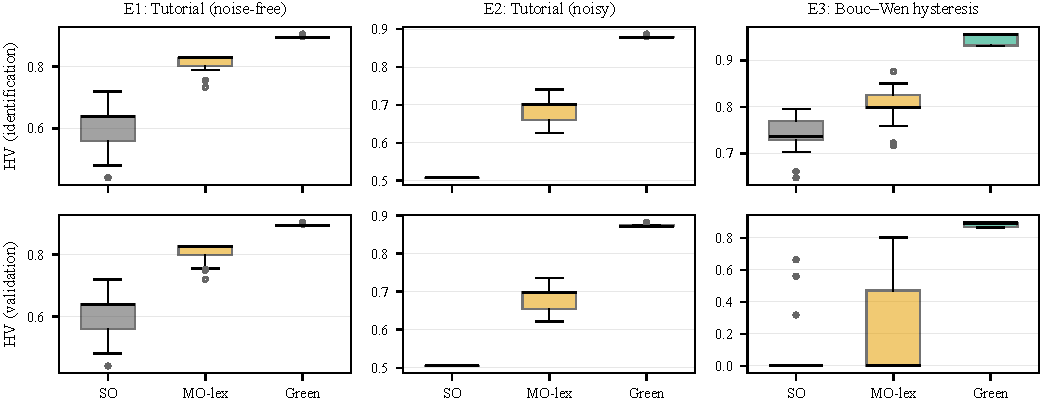
\includegraphics[width=\textwidth]{figures/fig_hv.pdf}\caption{Corrected equal-evaluation study: identification and validation hypervolumes of the delivered sets over 30 runs with $\rho=1$.}\label{fig:hv}\end{figure}
\begin{figure}[!htbp]\centering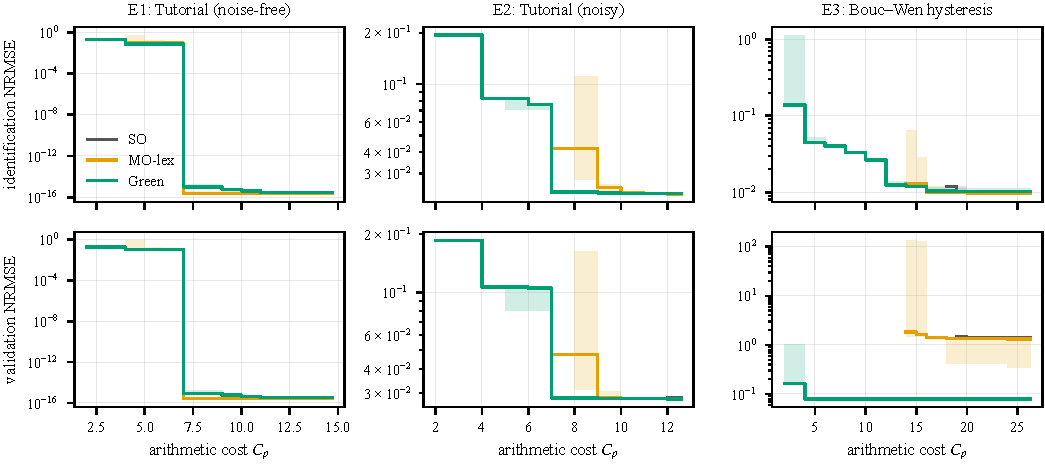
\includegraphics[width=\textwidth]{figures/fig_attainment.pdf}\caption{Median attainment curves and interquartile bands of the delivered sets in the corrected study.}\label{fig:attainment}\end{figure}
The selected Green costs are \EBGreenCsel, \ECGreenCsel{} and \EDGreenCsel{} operations, against \EBSOCsel, \ECSOCsel{} and \EDSOCsel{} for SO. On E1 all selected models are effectively exact; statistical differences below $10^{-14}$ have no practical accuracy interpretation. On noisy E2 the selected models do not recover the generating regressors, and the corrected Green sets do not retain the historical structure-recovery result. The earlier claim of full E2 recovery therefore does not apply to this study.

On E3, selection based only on identification error gives poor validation. The selected Green NRMSE is \EDGreenVALsel, compared with \EDSOVALsel{} for SO and \EDLexVALsel{} for MO-lex. Green sets contain models with substantially better validation, but the fixed $\tau$-rule does not choose them. Neither the rule nor its parameters are changed after observing validation. These outcomes prevent an accuracy-preserving interpretation of the E3 selected-model energy comparison.
Table~\ref{tab:models} makes the structural differences concrete for the declared representative runs. On E2, Green and MO-lex select the same three delayed regressors, whereas SO retains five. Similar validation errors therefore coexist with different operation counts. None of these representative structures is the three-regressor generating structure: prediction accuracy on the available record does not establish recovery of the original delays.

On E3, the representative Green model consists of seven linear delayed terms; the baselines also include a cubic product. Counting factors and coefficient multiplications distinguishes these structures more directly than counting terms alone. The representative Green model has a different cost from the across-run median because the representative is chosen by median validation NRMSE, not median cost. All three representative E3 models have poor free-run validation, consistent with the limitation of the fixed selection rule.
\begin{table}[!htbp]
\centering
\caption{Regressors of the model selected by the $\tau$-rule in the representative run (median validation NRMSE of the selected model) and its free-run validation NRMSE.}
\label{tab:models}
\setlength{\tabcolsep}{3pt}
\footnotesize
\begin{tabular}{llp{8.5cm}rr}
\toprule
Ex. & Method & Regressors & $C$ & NRMSE \\
\midrule
E2 & SO & $u(k) y(k-2),\ u(k-1),\ y(k-2),\ y(k-2)^{2},\ y(k-5)$ & 12 & 0.028 \\
E2 & MO-lex & $u(k-1),\ u(k-1) y(k-2),\ y(k-5)$ & 7 & 0.028 \\
E2 & Green & $u(k-1),\ u(k-1) y(k-2),\ y(k-5)$ & 7 & 0.028 \\
\midrule
E3 & SO & $u(k-2) u(k-4) y(k-3),\ u(k-6),\ u(k-7),\ u(k-8),\ y(k-1),\ y(k-2),\ y(k-7),\ y(k-8)$ & 18 & 1.413 \\
E3 & MO-lex & $u(k-3) u(k-4) y(k-2),\ u(k-6),\ u(k-7),\ u(k-8),\ y(k-1),\ y(k-2),\ y(k-8)$ & 16 & 1.418 \\
E3 & Green & $u(k),\ u(k-1),\ u(k-2),\ u(k-3),\ y(k-1),\ y(k-7),\ y(k-8)$ & 14 & 1.425 \\
\bottomrule
\end{tabular}
\end{table}

\subsection{Term and node ablations}
\begin{table}[!htbp]\centering
\caption{Corrected equal-evaluation ablation: medians over 30 runs with $\rho=1$.}
\begin{tabular}{llrrrrr}
\toprule
 &  & HV (id) & HV (val) & Cost & NRMSE & Evaluations \\
example & config &  &  &  &  &  \\
\midrule
\multirow[t]{5}{*}{E1} & Green & 0.896 & 0.893 & 7.000 & 0.000 & 4510.000 \\
 & MO-lex & 0.829 & 0.827 & 7.000 & 0.000 & 4510.000 \\
 & Pareto-nodes & 0.831 & 0.828 & 7.000 & 0.000 & 4510.000 \\
 & Pareto-terms & 0.896 & 0.893 & 7.000 & 0.000 & 4510.000 \\
 & SO & 0.640 & 0.640 & 9.000 & 0.000 & 4510.000 \\
\cline{1-7}
\multirow[t]{5}{*}{E2} & Green & 0.878 & 0.872 & 7.000 & 0.028 & 4510.000 \\
 & MO-lex & 0.702 & 0.699 & 10.000 & 0.028 & 4510.000 \\
 & Pareto-nodes & 0.812 & 0.807 & 11.000 & 0.028 & 4510.000 \\
 & Pareto-terms & 0.878 & 0.872 & 7.000 & 0.028 & 4510.000 \\
 & SO & 0.508 & 0.505 & 12.000 & 0.028 & 4510.000 \\
\cline{1-7}
\multirow[t]{5}{*}{E3} & Green & 0.955 & 0.893 & 16.000 & 1.420 & 4510.000 \\
 & MO-lex & 0.798 & 0.000 & 16.000 & 1.411 & 4510.000 \\
 & Pareto-nodes & 0.929 & 0.868 & 14.000 & 1.425 & 4510.000 \\
 & Pareto-terms & 0.954 & 0.893 & 16.000 & 1.189 & 4510.000 \\
 & SO & 0.736 & 0.000 & 18.500 & 1.394 & 4510.000 \\
\cline{1-7}
\bottomrule
\end{tabular}
\end{table}

The term-count ablation has no significant difference in validation hypervolume from Green on any tested example after Holm correction. Thus these experiments do not establish a consistent advantage of the arithmetic objective over term count, although arithmetic counting explicitly distinguishes additions and multiplications. The node objective assesses the full representation rather than the duplicate-free polynomial. Finite validation medians in the ablation table exclude failures: on E3, six term-ablation runs, one SO run and one MO-lex run fail validation under $\rho=1$. A smaller median among the remaining term-ablation runs must be interpreted alongside those failures.
\begin{figure}[!htbp]\centering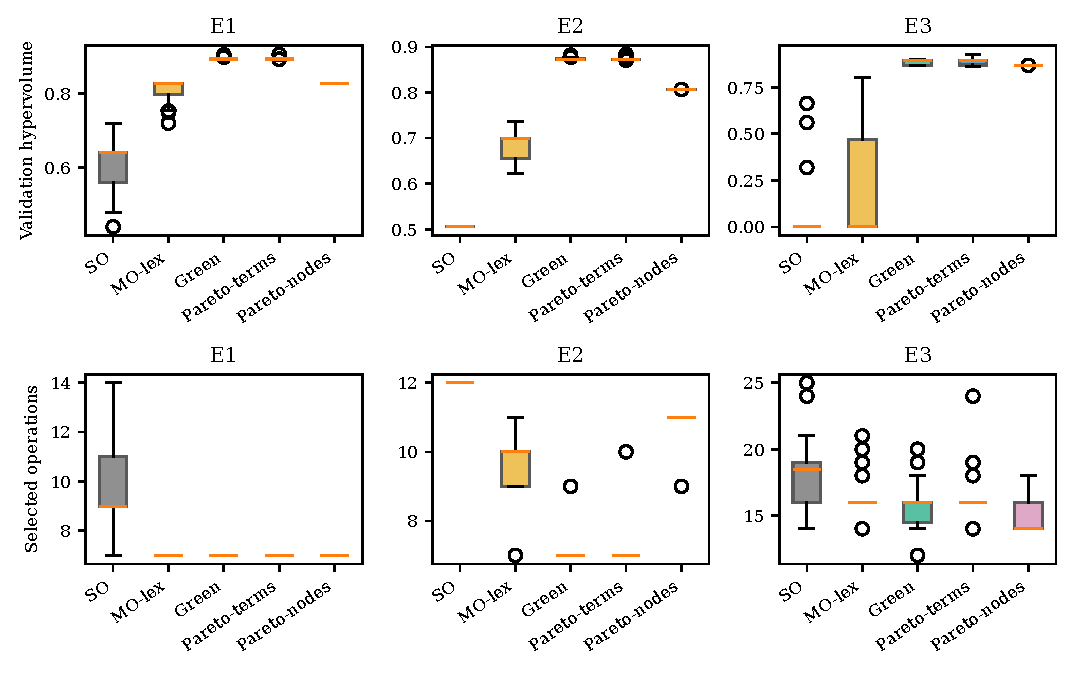
\includegraphics[width=\textwidth]{figures/fig_corrected_ablation.pdf}\caption{Equal-evaluation comparison with term and node objectives: validation hypervolume and selected arithmetic cost over 30 runs.}\end{figure}
\subsection{Multiplication-weight comparison}\label{sec:rho}
\begin{table}[!htbp]
\centering
\caption{Effect of the multiplication weight $\rho$ over 30 runs (medians). HV: identification hypervolume; $\Delta C_\tau$: reduction of the median selected cost of Green MGGP relative to SO, with the cost of the same scenario; $a{+}b$ and $C_{\rho_K}$: operation count and Karatsuba-weighted cost of the selected Green model; same: fraction of seeds in which Green MGGP selects the same structure under both weights.}
\label{tab:rho}
\setlength{\tabcolsep}{3.5pt}
\small
\begin{tabular}{llccccccc}
\toprule
 & & \multicolumn{3}{c}{HV$_\mathrm{id}$} & & \multicolumn{2}{c}{Green $\mathcal M_\tau$} & \\
\cmidrule(lr){3-5}\cmidrule(lr){7-8}
Ex. & weight & SO & MO-lex & Green & $\Delta C_\tau$ & $a{+}b$ & $C_{\rho_K}$ & same \\
\midrule
E1 & $\rho=1$ & 0.640 & 0.829 & 0.896 & 22\% & 7 & 48.6 & 100\% \\
 & $\rho_K$ & 0.738 & 0.884 & 0.929 & 20\% & 7 & 48.6 &  \\
\midrule
E2 & $\rho=1$ & 0.508 & 0.702 & 0.878 & 42\% & 7 & 48.6 & 80\% \\
 & $\rho_K$ & 0.622 & 0.773 & 0.910 & 43\% & 7 & 48.6 &  \\
\midrule
E3 & $\rho=1$ & 0.736 & 0.798 & 0.955 & 14\% & 16 & 109.5 & 0\% \\
 & $\rho_K$ & 0.819 & 0.874 & 0.969 & 14\% & 16 & 109.5 &  \\
\bottomrule
\end{tabular}
\end{table}

Both weights remain in the analysis. Table~\ref{tab:rho} reports the separate cost objectives and the fraction of identical selected Green structures. Changing $\rho$ changes relative structure costs, rather than merely rescaling them. Cost reductions in this table are reductions between method medians, not medians of per-run reductions; hypervolumes under different weights use different cost coordinates and cannot be treated as the same indicator. The weights were fixed before the corrected searches and are assessed by timing measurements in Section~\ref{sec:energy}.
\subsection{Theory and implementation checks}
\begin{table}[!htbp]
\centering
\caption{Empirical verification of Theorems~2 and~3 over 30 seeds. Lexicographic reduction: seeds in which SO and MO-lex produce identical populations in all generations; diverging seeds in which the divergence is preceded by an error tie between individuals of different cost, and in which the populations involved contain at least two individuals with $J_E=\infty$; median generation of the first divergence. Non-deterioration: largest $|U_t^1|$ over all runs and generations, bound $L(G,h)$ and population size $\mu$; runs with at least one decrease of the population-front hypervolume.}
\label{tab:checks}
\small
\setlength{\tabcolsep}{4pt}
\begin{tabular}{lcccccccccc}
\toprule
 & \multicolumn{4}{c}{Lexicographic reduction} & \multicolumn{3}{c}{Capacity} & \multicolumn{3}{c}{Runs with HV decrease} \\
\cmidrule(lr){2-5}\cmidrule(lr){6-8}\cmidrule(lr){9-11}
Ex. & identical & tie & $J_E{=}\infty$ & first div. & $\max|U_t^1|$ & $L(G,h)$ & $\mu$ & SO & MO-lex & Green \\
\midrule
E1 & 30/30 & 0/0 & 0/0 & -- & 8 & 50 & 100 & 30 & 30 & 0 \\
E2 & 30/30 & 0/0 & 0/0 & -- & 9 & 50 & 100 & 30 & 30 & 0 \\
E3 & 30/30 & 0/0 & 0/0 & -- & 10 & 260 & 100 & 30 & 30 & 0 \\
\bottomrule
\end{tabular}
\end{table}

Table~\ref{tab:checks} separates the two theoretical checks. Population hashes show identical SO and MO-lex trajectories in all 30 runs on each example for the primary weight, consistent with Theorem~\ref{thm:lex}; their delivered sets differ through final filtering. Green shows no population-front hypervolume decreases, and the observed union-front sizes satisfy the capacity condition of Theorem~\ref{thm:elitism}. These checks support the conditional theoretical statements rather than proving them for arbitrary searches. Canonical regression matrices of all 450 selected models across the five primary-weight configurations have full numerical column rank; this does not check every candidate evaluated during search.
\FloatBarrier
